% -- Encoding UTF-8 without BOM
% -- XeLaTeX => PDF (BIBER)

\documentclass[english]{cv-style}          % Add 'print' as an option into the square bracket to remove colours from this template for printing. 
                                    % Add 'espanol' as an option into the square bracket to change the date format of the Last Updated Text

\sethyphenation{english}{identification oriented processing manufacturing} % Add words between the {} to avoid them to be cut 

\exhyphenpenalty=10000
\hyphenpenalty=10000

\begin{document}

\header{Meili }{Vanegas-Hernandez}           % Your name
\lastupdated

%----------------------------------------------------------------------------------------
%	SIDEBAR SECTION  -- In the aside, each new line forces a line break
%----------------------------------------------------------------------------------------
\begin{aside}
%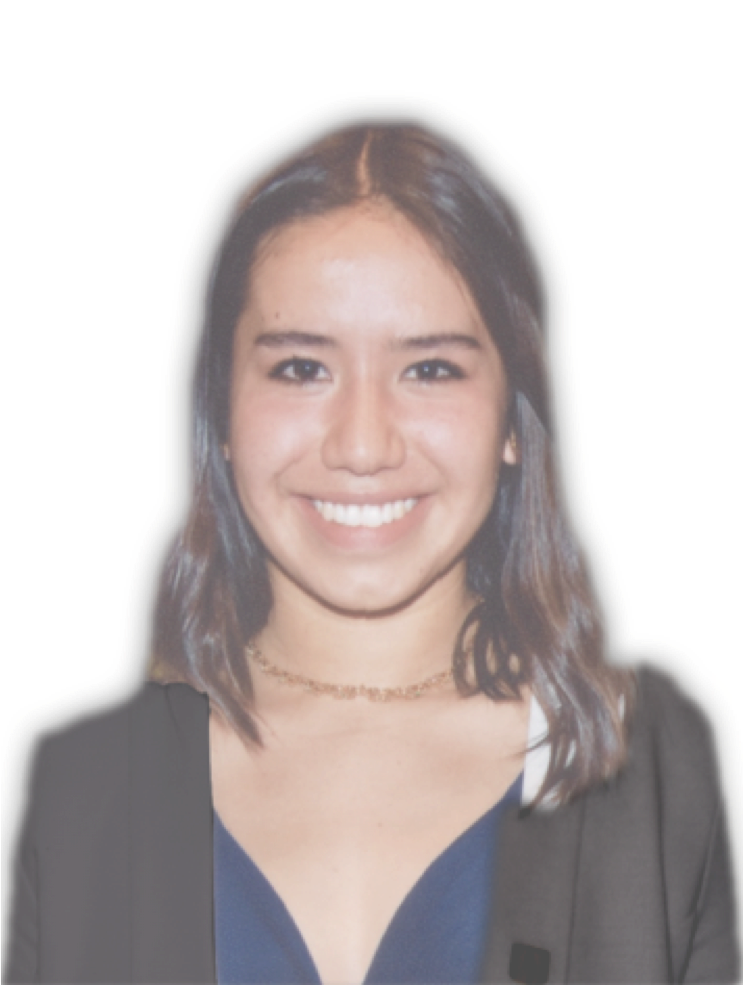
\includegraphics[width=3cm]{pictures/me.png}
%
\vspace{2.5cm}
\section{\textcolor{aquamarine}{contact}}\\
\vspace{0.2cm}
Bogota, Colombia\\
\vspace{0.1cm}
+57 (318) 489 2536\\
\vspace{0.1cm}
{\href{mailto:meilivh8@gmail.com}{\underline{meilivh8@gmail.com}}}\\
\vspace{0.1cm}
{\href{https://mvanegas10.github.io}{\underline{mvanegas10.github.io}}}\\
%
\vspace{2.5cm}
\section{\textcolor{aquamarine}{languages}}\\
\vspace{0.2cm}
Spanish (native)\\
\vspace{0.1cm}
English (proficient)\\
\vspace{0.1cm}
French (advanced)\\
\vspace{0.1cm}
German (beginner)\\
%
\vspace{2.5cm}
\section{\textcolor{aquamarine}{programming}}\\
\vspace{0.2cm}
{Python, JavaScript,\\
\vspace{0.1cm}
Java, C, SQL, Swift,\\
\vspace{0.1cm}
Matlab, \LaTeX{}, Visual\\
\vspace{0.1cm}
Basic, HTML, CSS}\\
\vspace{0.5cm}
{NodeJS, Jupyter\\
\vspace{0.1cm}
Notebooks, MongoDB,\\
\vspace{0.1cm}
Tablau, Django, D3.js,\\
\vspace{0.1cm}
AngularJS, ReactJS}\\
%
\end{aside}

%----------------------------------------------------------------------------------------
%	SKILLS SECTION
%----------------------------------------------------------------------------------------

\section{interests}
  \vspace{-0.2cm}
\textbf{professional:} analytics, visualization, data science, web developing, machine learning, big data, image analysis and processing, business intelligence, urban planning. \textbf{personal:} drawing, cycling, arts, hiking, photography, swimming, music.

%----------------------------------------------------------------------------------------
%	WORK EXPERIENCE SECTION
%----------------------------------------------------------------------------------------
 {\vspace{-0.4cm}}
\section{professional experience}

\begin{entrylist}
%------------------------------------------------
\entry
  {02.2019\\Present}
  {Steer}
  {Bogota, Colombia}
  {\jobtitle{Consultant}\\
  Participating in transit projects such as the 2019 Bogota's Mobility Survey and Transport Model.\\
  \bodyfontit{I developed a visual analytics tool that allows analysts to easily identify trips in trips matrices for several cities.} \\
    {\vspace{-0.09cm}}}
%------------------------------------------------
\entry
  {07.2017\\05.2018}
  {Computer Graphics \& HCI Group at TUK}
  {Kaiserslautern, Germany}
  {\jobtitle{Research Assistant}\\
  Designing and implementing a visual analytics tool to support failure detection in manufacturing processes.\\
  Master thesis: Developed BioCicle a \underline{\href{https://github.com/mvanegas10/BioCicle}{visual analytics tool}} to assist biological sequences identification and classification. \\
    {\vspace{-0.09cm}}}
%------------------------------------------------
\entry
  {01.2017\\07.2017}
  {ALIANZA CAOBA}
  {Bogota, Colombia}
  {\jobtitle{Researcher}\\
  Participating in a project along with the Secretary of Finance in Bogota to identify inaccurate taxpayers in real property taxes. \\ 
  Developing research activities, state-of-the-art review, data analysis and visualization.	\\
  \bodyfontit{I proposed a visualization that enabled easy outlier-detection in taxpayers.} \\
    {\vspace{-0.09cm}}}
%------------------------------------------------
\entry
  {06.2016\\07.2016}
  {I3S AND ESPACE LABORATORY AT SOPHIA ANTIPOLIS UNIVERSITY}
  {Nice, France}
  {\jobtitle{Junior Researcher}\\
  Working in the project Transport Oriented Modeling for urban denSification Analysis (TOMSA)/ECOS Nord. Building a urban decision support platform, which holds a Urban Agent-Based Model \textsc(ABM) to simulate the relocation of households under a spatial and possibilistic scenario and visualize multiple scenarios.\\
    {\vspace{-0.5cm}}}
%------------------------------------------------

\end{entrylist}

%----------------------------------------------------------------------------------------
%	EDUCATION SECTION
%----------------------------------------------------------------------------------------
 {\vspace{-0.5cm}}
\section{education}

\begin{entrylist}
%------------------------------------------------
\entry
{08.2017\\05.2018}
{M.Sc. Systems and Computing Engineering}
{Technische Universität Kaiserslautern}
{\bodyfontit{Emphasis in Applied Computing}\\
(\normalfont{International Exchange Program)}\\
{\vspace{-0.3cm}}}
%------------------------------------------------
\entry
{01.2017\\05.2018}
{M.Sc. Systems and Computing Engineering}
{Los Andes University}
{\bodyfontit{Emphasis in Applied Computing}\\
\normalfont{[GPA 4.30]}\\
{\vspace{-0.3cm}}}
%--------------------
%------------------------------------------------
\entry
{08.2012\\12.2016}
{B.Sc. Systems and Computing Engineering}
{Los Andes University}
{\normalfont{[GPA 4.08]}\\
{\vspace{-0.3cm}}}
%------------------------------------------------
\end{entrylist}

%----------------------------------------------------------------------------------------
%	OTHER QUALIFICATIONS SECTION
%----------------------------------------------------------------------------------------
 {\vspace{-0.5cm}}
\section{projects and contests}

\begin{entrylist}
%------------------------------------------------
\entry
{2016\\\vspace{-0.3cm}}
{Hackathon Cognitiva (Winner)}
{IBM, UniAndes, Alianza Caoba}
{\vspace{-0.3cm}}
%------------------------------------------------
\entry
{2015\\\vspace{-0.3cm}}
{IT Innovation Contest (Second Place)}
{Los Andes University}
{\vspace{-0.3cm}}
%------------------------------------------------
\entry
{2012\\\vspace{-0.5cm}}
{Summa Cum Laude}
{Gimnasio Vermont}
{\vspace{-1cm}}
%------------------------------------------------
\end{entrylist}
{\vspace{-0.1cm}}
\section{publications}

\begin{entrylist}
%------------------------------------------------
\entry
{08.2017\\\vspace{-0.3cm}}
{A new urban segregation-growth coupled model using a belief-desire-intention possibilistic framework}
{WI '17 Proceedings. Leipzig, Germany}
{\vspace{-0.3cm}}
%------------------------------------------------
\end{entrylist}

\end{document}